\section{Resultados}
%Deben incluir los resultados de los experimentos, utilizando el formato más adecuado
%para su presentación. Deberón especificar claramente a qué experiencia corresponde
%cada resultado. No se incluirán aquí corridas de máquina. Algo fundamental en su
%aprendizaje en la materia es la presentación de resultados de forma clara y concisa para
%el lector.



\subsection{Experimento 1}
Se procedio a ejecutar el método de kNN variando k, para K = 2, 10 y 20 con k $\in$ $\{$2, 30, 100, 500$\}$ 
Los resultados obtenidos fueron los siguientes:
\begin{itemize}
\item Con K = 2\\
\item Con K = 10\\
    \begin{figure}[H]
    \centering
    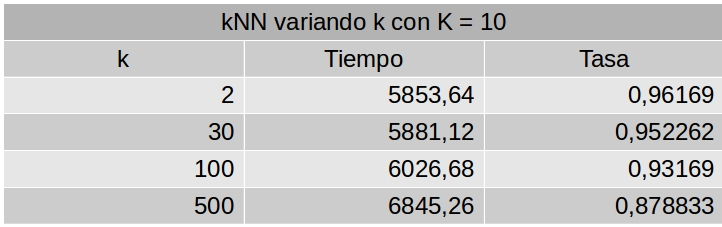
\includegraphics[scale=0.5]{Tablas/kNNK10.jpg}\caption{La tasa es el promedio de las tasas de cada partición}
    \end{figure}

    \begin{figure}[H]
    \centering
    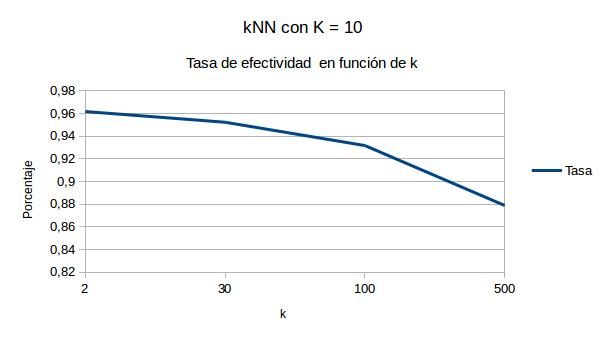
\includegraphics[scale=0.7]{Graficos/graficoknnK10.jpg}
    \end{figure}

\item Con K = 20\\
\end{itemize}

\subsection{Experimento 2}
Se procedio a ejecutar el método de kNN+PCA variando $\alpha$, para K = 2, 10 y 20 con k = 2.\\ 
Los resultados obtenidos fueron los siguientes:
\begin{itemize}
\item Con K = 2\\

    
\item Con K = 10\\

\item Con K = 20\\
\end{itemize}

\subsection{Experimento 3}


\subsection{Competencia Kaggle}
Para realizar nuestro submission en la página de Kaggle, a la competencia de Digit Recognizer, modificamos levemente el codigo de nuestro programa. El mismo se encuentra en la carpeta Kaggle. Las modificaciones se deben a que en este caso, la base de test proporcionada por la página no tiene labels, no utilizamos el método de K-Fold Cross Validation, la funcion kNN ahora tiene que devolver las predicciones de los dígitos, entre otras cosas.\\
Luego de toda la experimentación concluímos que los mejores parámetros, en cuanto tiempo y eficacia, para correr el programa son:
\begin{itemize}
\item $\alpha$ = 
\item $k$ = 
\end{itemize}

El sistema de Kaggle nos proporciono que tuvimos una tasa de efectividad del XX, al trata de reconocer la base de test de 28.000 dígitos